\documentclass[12pt]{report}
\usepackage[utf8]{inputenc}
\usepackage[czech]{babel}
\usepackage{hyperref}
\usepackage{graphicx} 
\usepackage{float}
\usepackage{blindtext}
\usepackage{enumitem}
\usepackage{scrextend}
\title{Logické řízení - řízení kotle na ohřev vody}
\author{Jan Kohlíček}

\begin{document}

\begin{titlepage}
\begin{flushleft} 
{\includegraphics[width=.5\textwidth]{./images/fav_logo.jpg}\\[3cm]}
\end{flushleft}
\begin{center}

{\Huge KIV/TI - Semestrální práce}
\\[0.3cm]
\vspace{1.7cm}
{\Large Kateřina Kratochvílová - A13B0364P}\\
\vspace{0.2cm}
{\normalsize dtwok8@students.zcu.cz}\\
\vspace{1cm}
{\Large Jan Kohlíček - A13B0350P}\\
\vspace{0.2cm}
{\normalsize kohl@students.zcu.cz }
\vfill
{\large \today}
\end{center}
\end{titlepage}

\tableofcontents
\thispagestyle{empty}



\chapter{Zadání}
\setcounter{page}{1}
Navrhněte konečněautomatový model pro řízení kotle na ohřev vody podle zadání:\\
\\
Po stisknutí tlačítka START obsluhou systém začne napouštět kotel a po dosažení určité minimální úrovně hladiny zapne topné spirály. Po dosažení maximální hladiny kotle přestane napouštět a dokončí ohřev. Po dosažení stanovené teploty dojde k vypnutí topných spirál. Předpokládáme kontinuální odběr teplé vody, kotel musí být schopen vodu dopouštět.\\
\\
Definujte potřebné vstupní a výstupní signály, automat popište přechodovým grafem.\\
\\
Model řídícího automatu realizujte softwarově na základě principů popsaných v materiálu. Všechny signály od čidel modelujte vstupy od klávesnice, řídicí signál a informaci o stavu vypisujte textově na obrazovku.\\


\chapter{Analýza úlohy}
Kotel bude přijímat impulsové signály od čidel hladinoměru a teploměru. Vždy bude moci přijmout jen \textbf{jeden signál}, na který může reagovat vysláním \textbf{neomezeným počtem signálů}.
Za těchto podmínek lze použít konečný automat \textbf{Mealyho typu}.\\
Stavy, kterými může kotel během celého cyklu projít: nečinnost, start, napouštění - málo vody, topení, napouštění - topení, napuštění - dost vody na topení ale netopí se, teplota OK hladina OK, Plná nádrž -netopí se nenapouští se\\

Vstupní signály: 
\begin{itemize}
\item HL1 - málo vody na topení
\item HL2 - dost vody na topení
\item HL3 - plná nádrž
\item TP1 - teplota klesla pod minimální úroveň
\item TP2 - teplota je na maximu
\end{itemize}

Výstupní signály: 
\begin{itemize}
\item ZN - zapni napouštění
\item VN - vypni napouštění
\item ZT - zapni topení
\item VT - vypni topení
\end{itemize}



\begin{figure}[h]
		\centering
		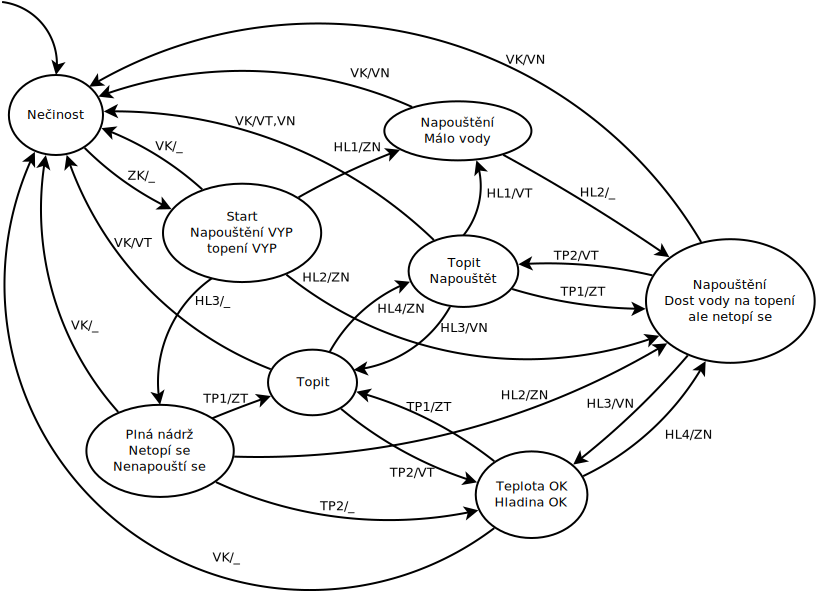
\includegraphics[width=\textwidth]{./images/graf.png}	
		\caption{Návrh konečného automatu}
\end{figure}

\chapter{Implementace}
Simulace kotle je řešená jako \textbf{konzolová aplikace}, napsaná ve skriptovacím jazyce \textbf{Python}. Tento jazyk byl zvolen pro jeho produktivnost z hlediska rychlosti psaní kódu.\\

\section{Adresářová struktura}
	Aplikace má následující adresářovou strukturu:\\
	\begin{description}
	\item [boiler\_controller:] složka modulu

	\begin{description}
		\item [\_\_main\_\_.py:] Spouští automat.
		\item [finite\_automata.py:] Třída obsahuje nekonečný cyklus ve kterém se spouští jednotlivé stavy, dále obsahuje šablonu pro stavy, která zajišťuje vstup od uživatele a výpis informací.
		\item [signals.py:] Soubor obsahuje dvě enum množiny vstupních a výstupních signálů.
		\item [states.py:] Třída se statickými metodami, co metoda to jeden stav. Metody mají jeden parametr vstupní signál a vrací dvě hodnoty následující stav a pole výstupních signálů.
		
	\end{description}	
	\item [docs:] Dokumentace semestrální práce.			
	\item [setup.py:] Vytvoření balíčků (PyPI).
	\end{description}

\chapter{Uživatelská příručka}
\section{Spuštění aplikace}
Pro spuštění je potřeba mít nainstalovaný Python, který lze stáhnout z \url{https://www.python.org/downloads/}\\
Aplikaci spustíte ve složce projektu příkazem \texttt{"python boiler\_controller"} na linuxu \texttt{"python3 boiler\_controller"}.\\
\\
Volitelné parametry:
\begin{itemize}
	\item \texttt{-h} ... vypíše nápovědu
	\item \texttt{-v} ... vypíše verzi
\end{itemize}

\section{Ukázka}

\begin{figure}[h]
		\centering
		\includegraphics[width=0.8\textwidth]{./images/app_start.png}	
		\caption{Start aplikace}
\end{figure}

\begin{figure}[h]
		\centering
		\includegraphics[width=0.8\textwidth]{./images/app_progress.png}	
		\caption{Průběh aplikace}
\end{figure}

\begin{figure}[h]
		\centering
		\includegraphics[width=0.8\textwidth]{./images/app_error.png}	
		\caption{Stav CHYBA při neplatném vstupním signálu}
\end{figure}

\chapter{Závěr}
V semestrální práci jsme vytvořili návrh automatu a jeho následnou implementaci.
Překvapilo nás, jak bylo obtížné a časově náročné navrhnout konečný automat, který by měl mít praktické použití. Tato zkušenost nám pomohla pochopit výhody a nevýhody konečných automatů.


\end{document}